\documentclass[a4paper, 11pt]{article} % Font size (can be 10pt, 11pt or 12pt)

\usepackage[protrusion=true,expansion=true]{microtype} % Better typography
\usepackage{graphicx, grffile} % Required for including pictures
\usepackage{hyperref} % Clickable cross-referencing

\usepackage{mathpazo} % Use the Palatino font
\usepackage{amsmath} % Gets \text{} working in math mode.
\usepackage[T1]{fontenc} % Required for accented characters
\linespread{2} % Change line spacing here, Palatino benefits from a slight increase by default
\usepackage[margin=1.5in]{geometry}
\usepackage{changepage}
\usepackage{collectbox}

\makeatletter
\newcommand{\sqbox}{%
	\collectbox{%
		\@tempdima=\dimexpr\width-\totalheight\relax
		\ifdim\@tempdima<\z@
		\fbox{\hbox{\hspace{-.5\@tempdima}\BOXCONTENT\hspace{-.5\@tempdima}}}%
		\else
		\ht\collectedbox=\dimexpr\ht\collectedbox+.5\@tempdima\relax
		\dp\collectedbox=\dimexpr\dp\collectedbox+.5\@tempdima\relax
		\fbox{\BOXCONTENT}%
		\fi
	}%
}
\makeatother

\makeatletter
\renewcommand\@biblabel[1]{\textbf{#1.}} % Change the square brackets for each bibliography item 
%from '[1]' to '1.'
\renewcommand{\@listI}{\itemsep=0pt} % Reduce the space between items in the itemize and 
%enumerate environments and the bibliography
\renewcommand{\sectionautorefname}{\S}

\renewcommand{\maketitle}{
\begin{flushright}
	{\LARGE\@title}
	\vspace{50pt} \\
	{\large\@author}
	\\\@date
	\vspace{40pt}
\end{flushright}
}

\title{
	\begin{figure}
		\begin{center}
					
\includegraphics[width=8cm]{figures/logo.jpg}
		\end{center}
	\end{figure}	
	\textbf{ST2288 UROPS Report
}\\
Applying machine learning techniques to determine the occupancy of parking lots}

\author{\textsc{Rayakar Achal Ajeet, A0156139B}\\
		\textit{National University of Singapore}
}

\date{27th April, 2018}

%----------------------------------------------------------------------------------------

\begin{document}

\maketitle % Print the title section

\newpage

\tableofcontents

\newpage

\section{Summary}
    This report discusses the current state of the UROPS project entitled ``Parking Lot Classification''; 
    namely, it details our motivations, literature and tools utilized, and results on a public parking lot 
    dataset. It then proceeds to describe the manner in which we intend to use the tools we are 
    developing to serve NUS parking lot users in real-time.

\section{The problem}
    The environmental impact and wastage of time attributable to drivers searching for parking space 
    can be non-trivial: congestion caused by such drivers accounts for between 8\% and 74\% of traffic 
    in American cities \cite{pollution-paper}\relax. In the Singaporean context, many parking lots are 
    multi-storey in nature. When parking is scarce, traversal through such lots can be a great 
    inconvenience. Currently, Singaporean parking lots are equipped with occupancy signboards of the 
    following kind:
    \vskip 5mm
    \begin{figure}[h]
        \centering
        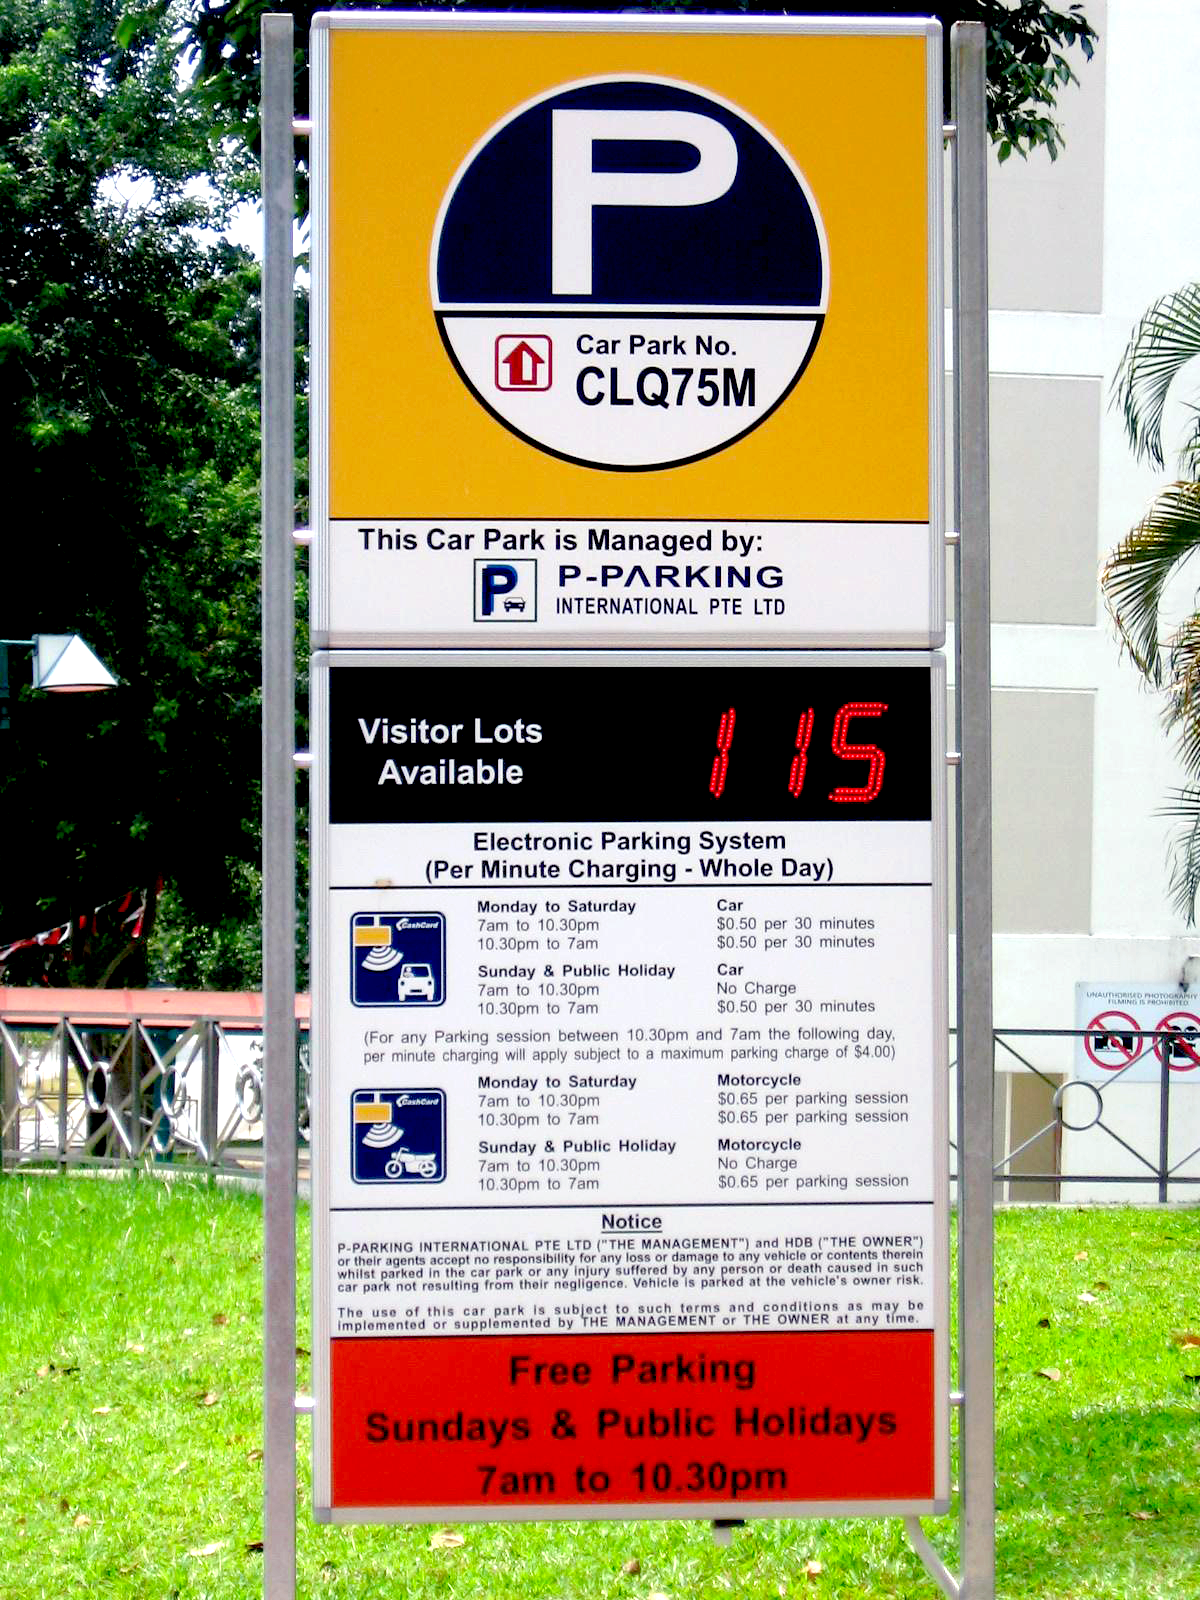
\includegraphics[width=4cm]{figures/curr_sign.png}
        \caption{A typical occupancy signboard.}
    \end{figure}
    \newpage
    While these signboards give users \textit{aggregate} information on the state of the parking lot, 
    more granular detail would be beneficial--if users knew exactly which parking spots were available, 
    they would save time otherwise spent looking for them. 
    
    Currently, solutions to make information available to users more granular include low-power sensors 
    installed spot-wise. These sensors connect to the Internet to communicate to lot managers and 
    users the occupancy status of each spot. While this Internet of Things-based idea is both simple 
    and likely reliable, \textit{city-wide} installation and maintenance of such devices may involve 
    significant cost.
    \vskip 5mm
    \begin{figure}[h]
    	\centering
    	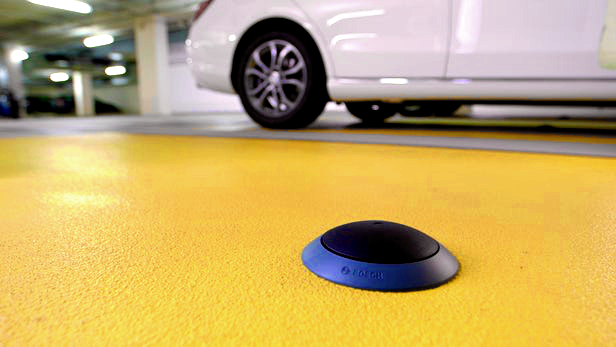
\includegraphics[width=8cm]{figures/sensor.jpg}
    	\caption{An infrared and magnetic-based parking sensor~\cite{parking-sensors}\relax.}
    \end{figure}
    We therefore wanted to find a way to deliver users this same information through means that 
    maximize the use of current infrastructure, such as the expansive network of CCTVs monitoring 
    Singaporean parking lots. Namely,
    \vskip 1mm
    \begin{center}
        \textbf{
        how can one use the \textit{image} of a parking lot to determine its spot-wise occupancy, and then deliver this information to users, in real-time?
        }
    \end{center}

\section{Our tool}
    There are several machine learning techniques available to users in the domain of computer vision, 
    with convolutional neural networks (CNNs) being state-of-the-art for image classification problems. 
    Since our problem is of this nature (given the image of a spot, determine if it is occupied or not), we 
    have chosen to learn about and deploy them for our purposes. This section offers a brief 
    explanation of how CNNs work. Firstly, and more generally, we consider artificial neural networks 
    (ANNs).
    
    \hspace*{-6mm}\textbf{Neural networks: statistical models}
    
    In one sentence: ANNs, of which CNNs are one kind, are statistical models that are created using 
    supervised learning algorithms.
    
    These algorithms process input, create output, and alter the model to produce output closer to the 
    expected (\textit{true}) output. In the case of occupancy detection, this would mean altering the 
    model to more accurately ascertain which spots are occupied and which are not. This iterative 
    process of alteration is called \textit{training} the model.
    
    The utility of the model is in its predictive power: given new inputs for which we may not know the 
    correct output, the model can create accurate predictions if adequately-trained. In our case, this will 
    come into play when serving users with a prediction of spot occupancy. \\
    \textbf{An analogue to the human brain~\cite{brain-analogy}} \\
    \hspace*{6mm}
    The human brain's neural networks are comprised of \textit{neurons} connected to each other for 
    the transmission of electrochemical signals. Similarly, ANNs are comprised of artificial neurons that 
    transmit numerical information to one-another through artificial synapses, which weight the 
    information:
    \vskip 5mm
    \begin{figure}[h]
        \centering
        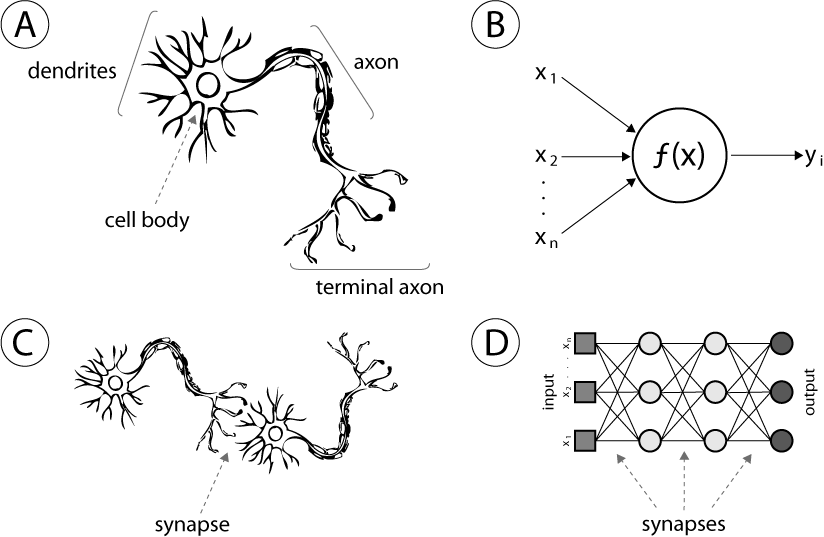
\includegraphics[width=12cm]{figures/analogy.png}
        \caption{In both cases, ``dendrites'' control input, ``synapses'' output, and ``cell bodies'' 
        calculate.}
        \vspace{5mm}
        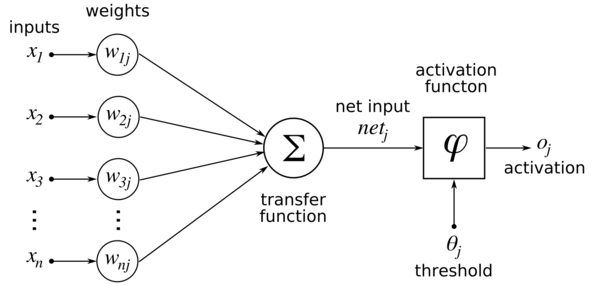
\includegraphics[width=8cm]{figures/neuron.png}
        \caption{A closer look at the artificial neuron.}
    \end{figure}

	The artificial neuron $j$ finds $\Sigma_{i = 1}^{n}x_{i}w_{ij}$, the \textit{net input}, and applies an 
	\textbf{activation function} to it, usually a rectifier ($f(x) = x^+$). The purpose of the rectifier, in 
	non-technical terms, is to help the model train faster--i.e., to improve its predictions more quickly 
	than it would without it~\cite{use-of-relu}. From this activation function comes the output 
	of the neuron, which is then passed to another.

    \hspace*{-6mm}\textbf{Artificial neurons in context: the network itself~\cite{cnn-working}\relax} 
    
    This context will be provided by considering the workings of a CNN in a binary classification 
    problem similar to ours: that of differentiating between X's and O's. The following is a view of the 
    possible structure of this CNN; each component will be explained:

     \begin{figure}[h]
       	\centering
       	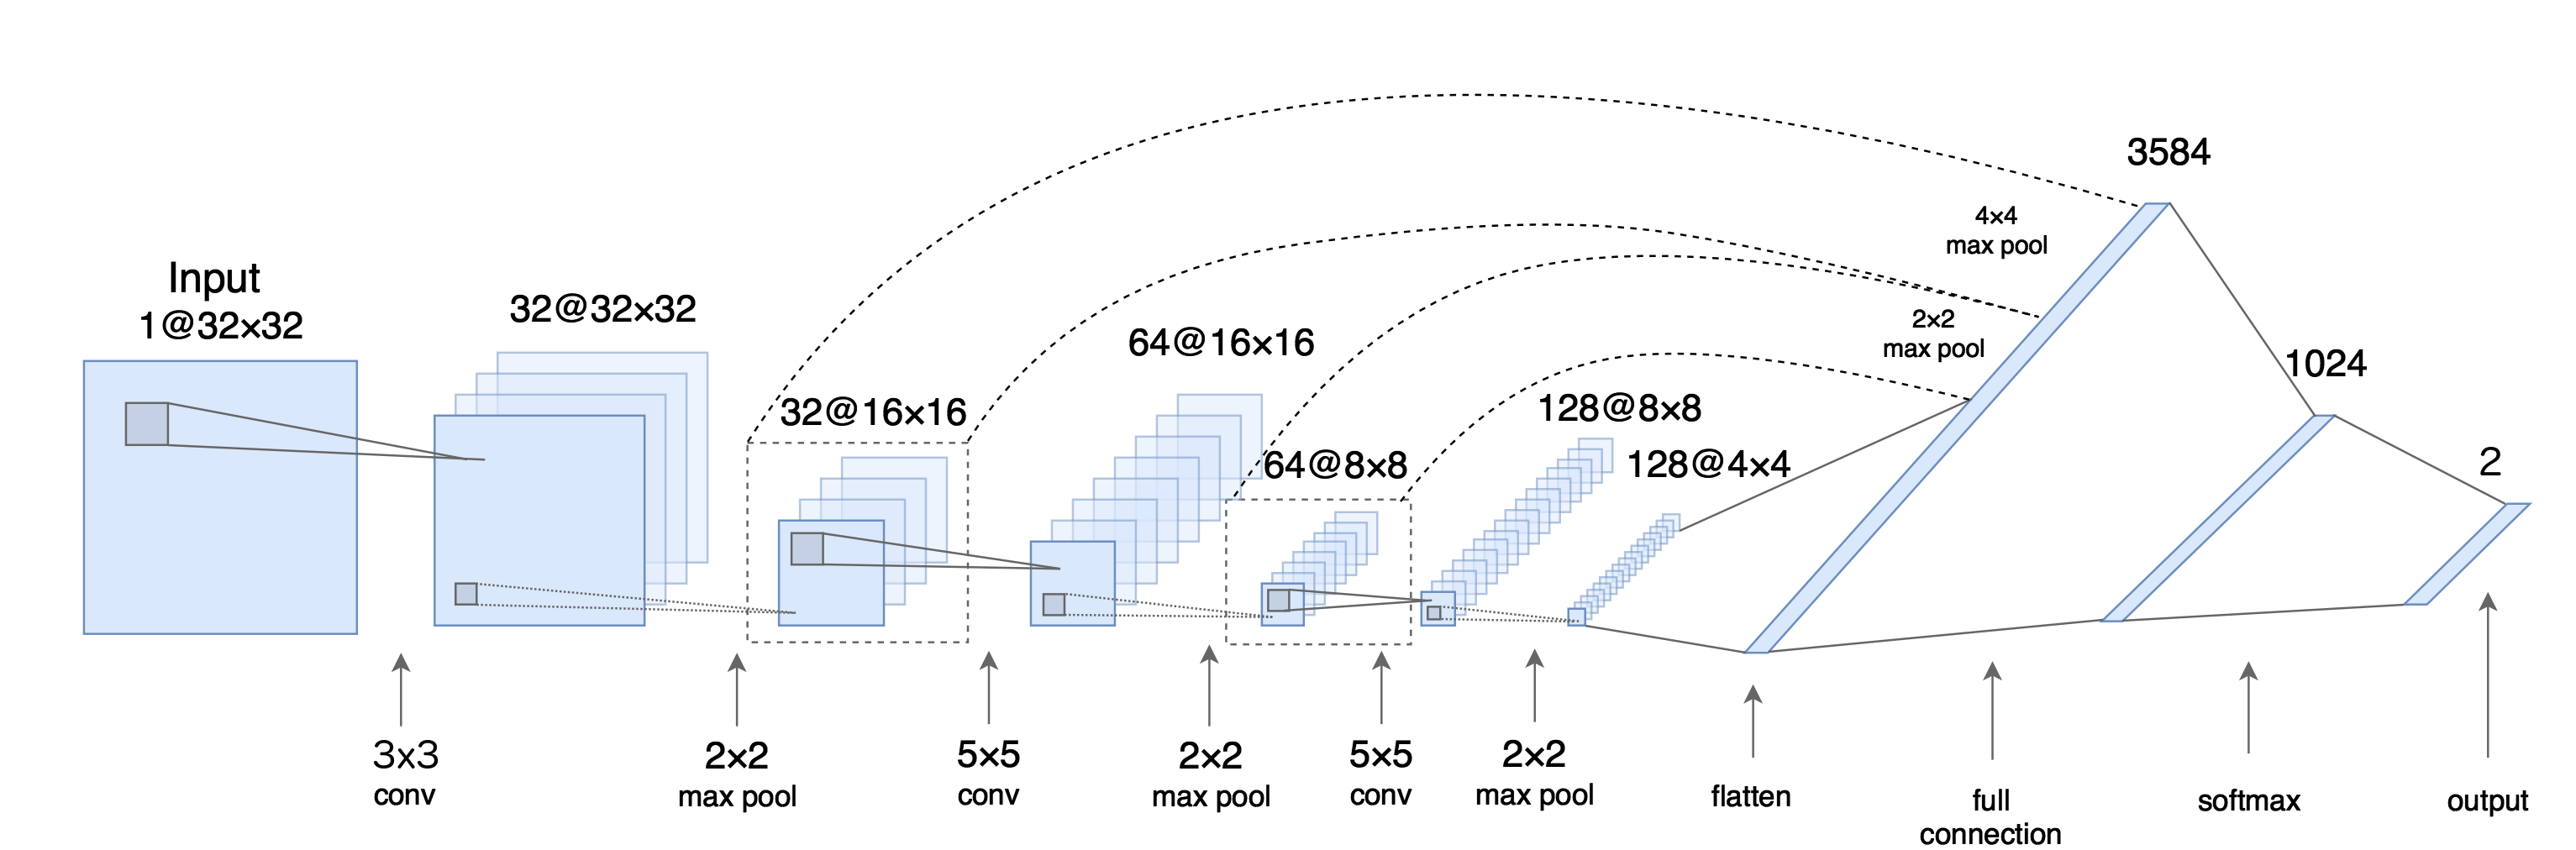
\includegraphics[width=14cm]{figures/architecture.png}
       	\caption{The structure, or \textit{architecture} of this CNN~\cite{architecture}\relax.}
       	\label{archi}
    \end{figure}

    The CNN takes the picture of an ``X'' or ``O'' as the input. Given that this input is digital, it will 
    be represented numerically, by pixels:
    \vskip 5mm
    \begin{figure}[h]
       	\centering
       	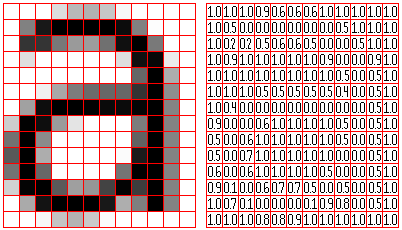
\includegraphics[width=6.5cm]{figures/pict_num.png}
       	\caption{A grayscale ``a'', numerically-represented: black is 0, white, 1~\cite{pict-num}\relax.}
    \end{figure}
 		
 		Suppose that our images are 32-by-32 pixels wide, meaning they can be represented by
 		two-dimensional arrays as above. After the input of such an image, it is passed to a 
 		\textbf{convolutional layer}. This convolutional layer extracts, in this case, 32 \textbf{feature 
 		maps} from the image. 
 		These feature maps are used to characterize the image in a manner that allows for ``X's'' and 
 		``O's'' to be distinguished, even if the input images are distorted in some way:
 		\vskip 5mm
 		\begin{figure}[h]
 			\centering
 			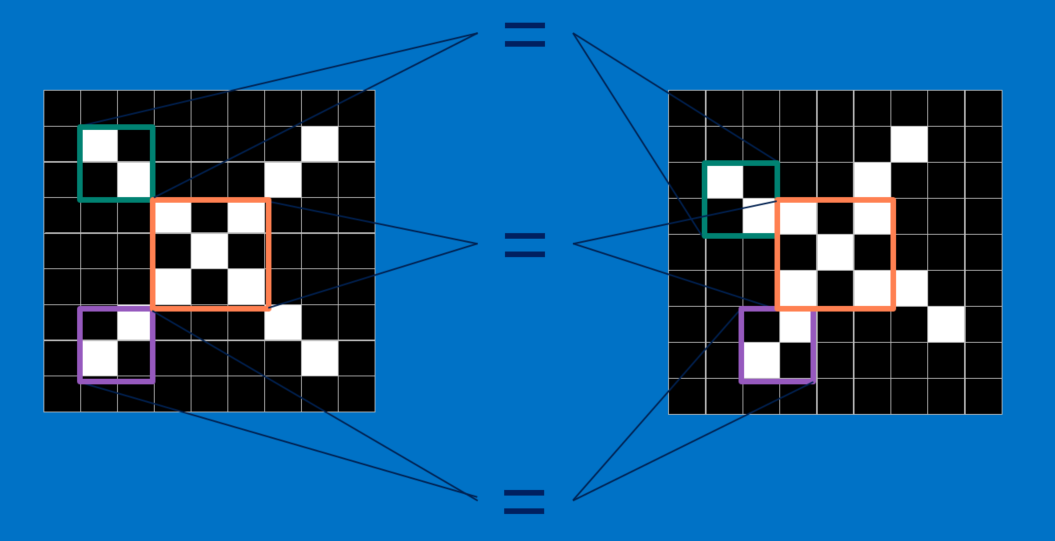
\includegraphics[width=8cm]{figures/explan_3.png}
 			\caption{Suppose the highlighted are the characterizing features of an ``X''.}
 		\end{figure}
 
 		This extraction occurs through the use of \textbf{filters}, which are (in this case) 3-by-3
 		numerical arrays. The elements of these arrays are selected by the CNN automatically, and 
 		change through the training process. This procedure of change will be revisited in the discussion 
 		of \textbf{backpropagation}. Of current concern are the filters and the convolution process itself. 
 		This process involves convolving the filter with each 3-by-3 ``patch'' of the image array, as 
 		shown:
% 		\vskip 5mm
 		\begin{figure}[h]
 			\centering
 			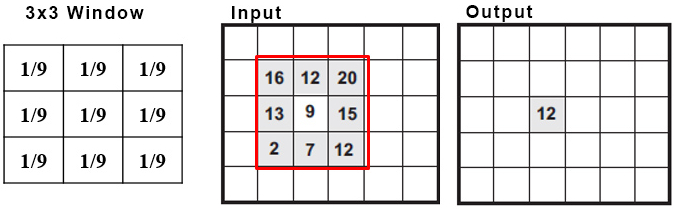
\includegraphics[width=7.5cm]{figures/filter_convol.jpg}
 			\caption{Convolving the filter with one 3-by-3 region of the input~\cite{convol-filter}\relax.}
 		\end{figure}
 		\begin{figure}[h]
 		\centering
 		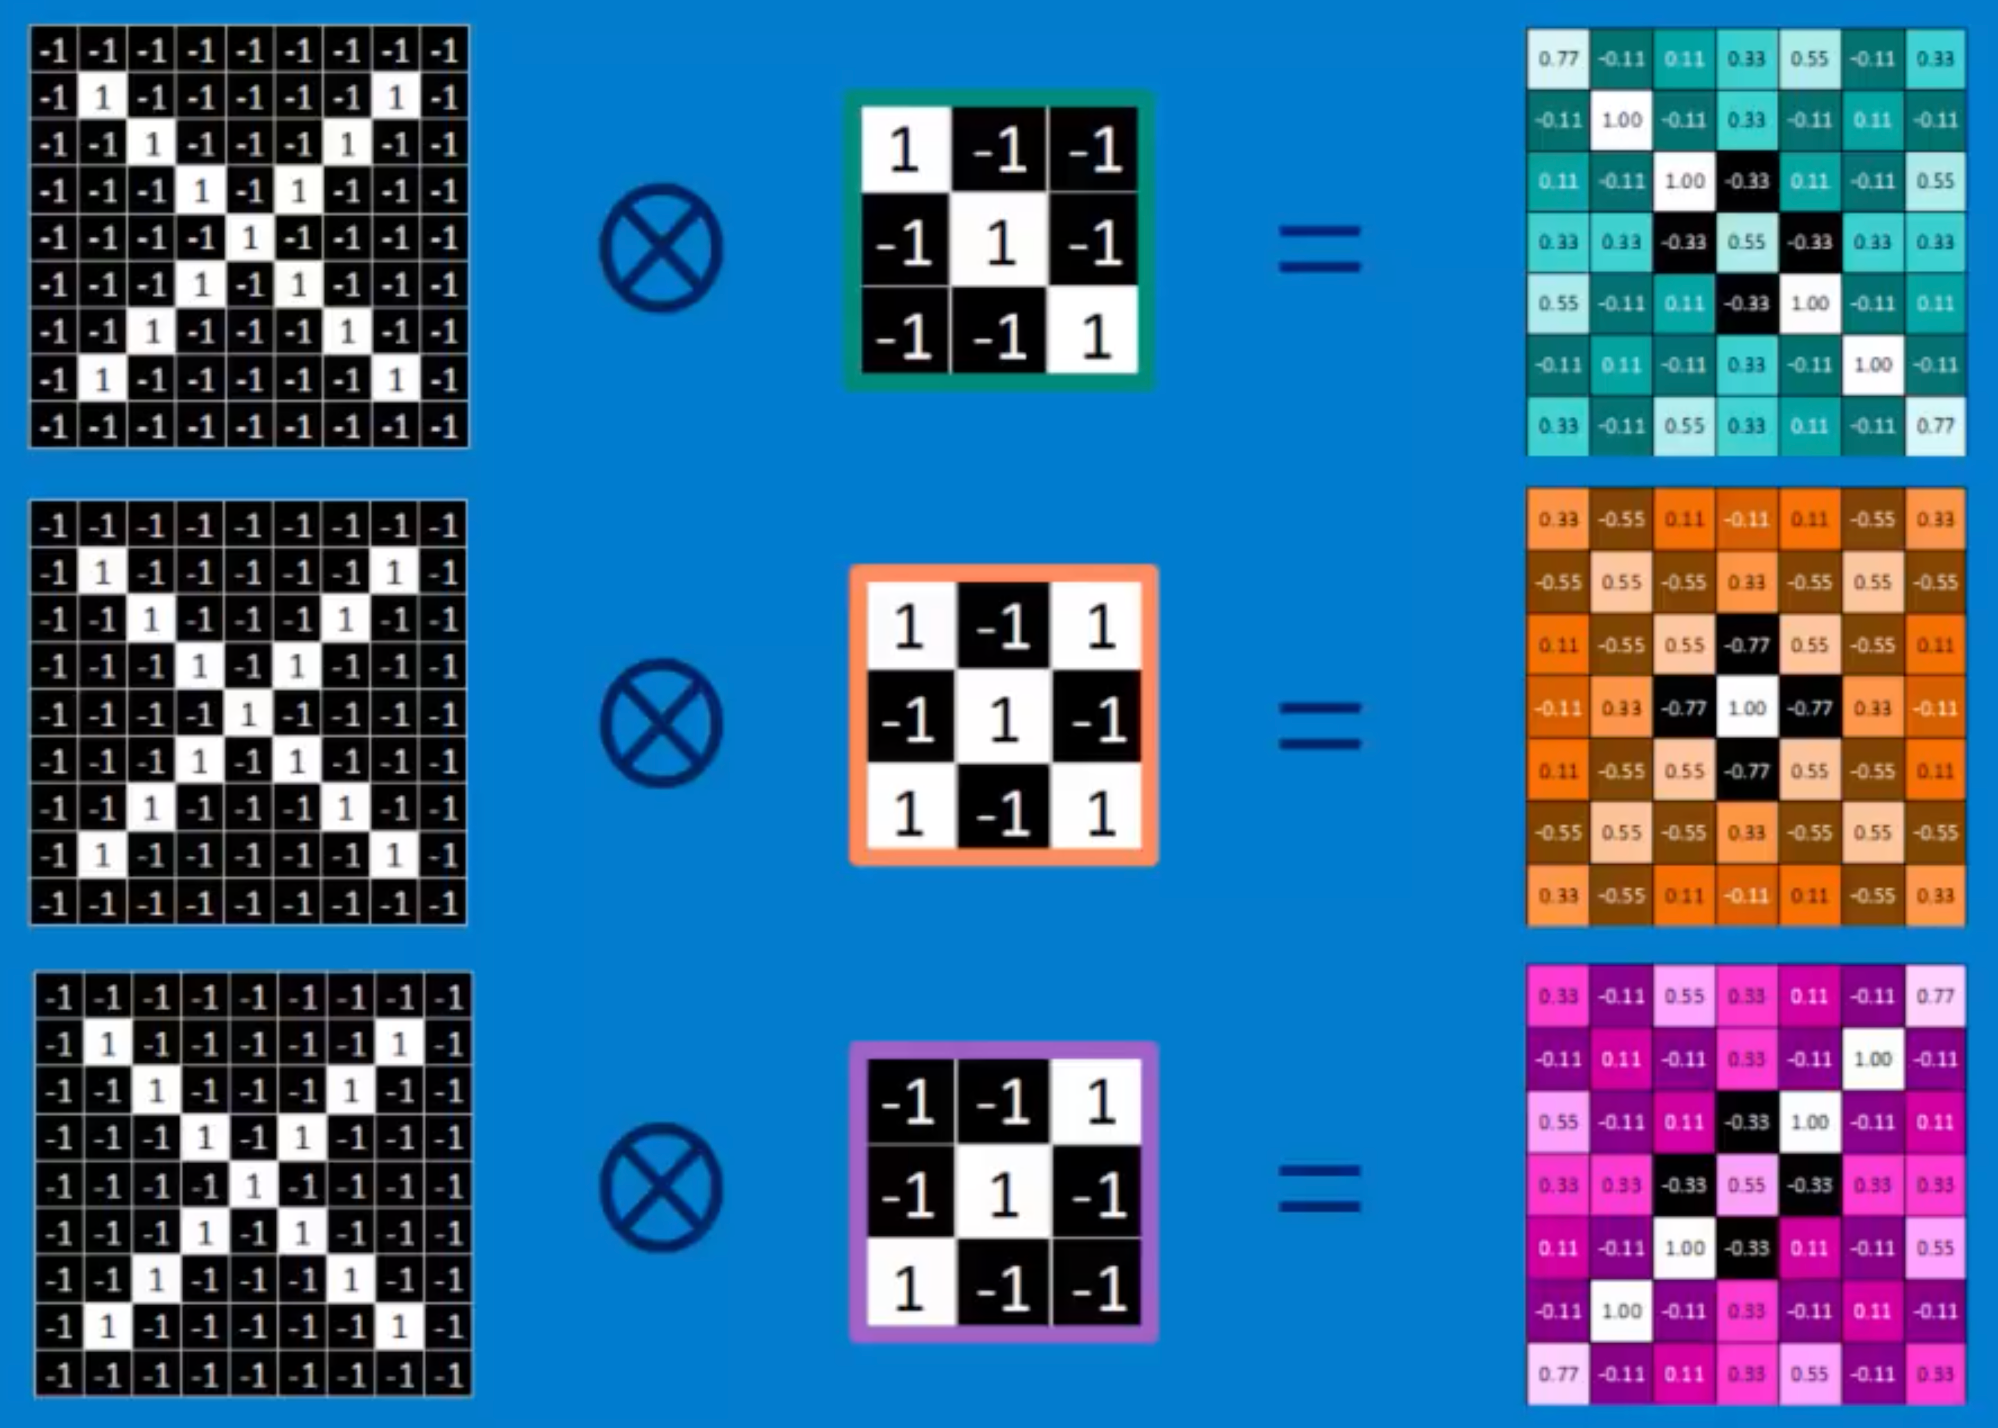
\includegraphics[width=6cm]{figures/output_vol.png}
 		\caption{Each filter searches for something else in the image, and the result of the convolution 
 			represents this numerically if it is found.}
 		\end{figure}
 		\newpage
 		An output \textit{volume} is obtained after the image is passed through the first convolution 
 		layer; this volume consists of 32 feature maps that take the form of 32-by-32 arrays. Each 
 		feature 
 		map represents the result of the convolution of a specific filter with the image. Presumably, each 
 		filter searches for a different characterizing property of the image. An intuitive idea of what filters 
 		may ``look for'' is given by the following image; in a CNN being used for facial recognition, the 
 		filters may be \textbf{weighted in such a manner} that they each focus on a particular 
 		characterizing feature of the human face: the eyes, nose, lips, etc.: 
 		\vskip 5mm
 		\begin{figure}[h]
 			\centering
 			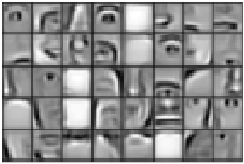
\includegraphics[width=6cm]{figures/filter_int.png}
 			\caption{Each segment of this image represents what pattern of pixels a filter may be ``looking 
 			for''.}
 		\end{figure}
	
	An immediate issue with the creation of this first output volume is the dimensionality of the data: 
	given CNNs have numerous convolutional layers (intuitively, each one leads to a more precise 
	characterization of the image), convolving can become increasingly computationally-expensive as 
	inputs increase in size. This is the motivation for the \textbf{pooling layers} found in CNNs. 
	
	In the case of this network, pooling is conducted using 2-by-2 arrays, which traverse each 32-by-32 
	filter map produced by the convolutional layer, to create an output volume that is of the dimensions 
	32-by-16-by-16; that is, each feature map in this volume is reduced in size. This traversal involves 
	compression of each map by retaining only the maximum value present under the traversing array; 
	this is known as \textbf{max pooling}, and is generally known to be an effective manner in which to 
	reduce volume size without excessive loss in the accuracy of the CNN. The following visualizes a 
	snapshot of this process:
	\vskip 5mm
	\begin{figure}[h]
		\centering
		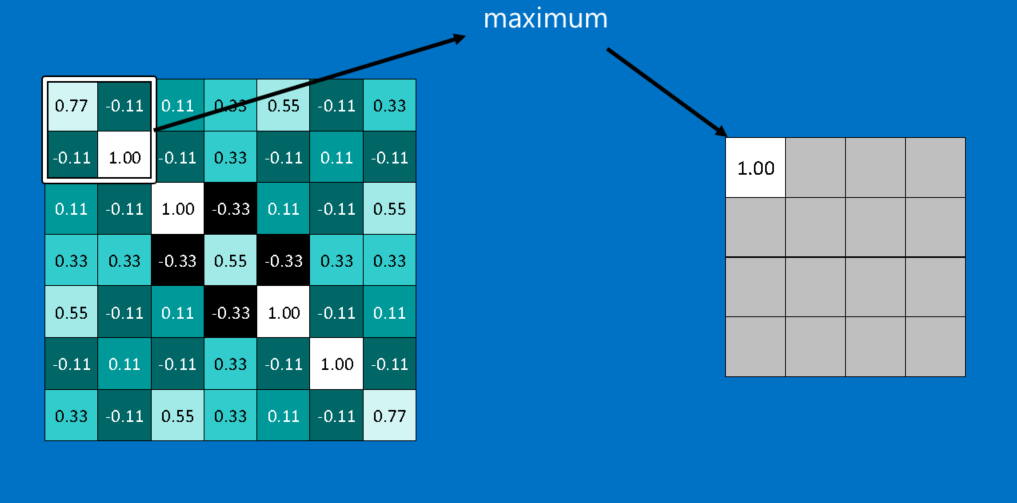
\includegraphics[width=8cm]{figures/pooling.png}
		\caption{Only the maximum value is retained.}
	\end{figure}

	The final procedure in this sequence is the application of the activation function: rectification using 
	the Rectified Linear Unit (ReLU), as aforementioned. It leaves the dimensions of the volume passed 
	to it unchanged. 
		
	This sequence of computations is done repeatedly in a CNN. In the case of this example, three 
	times. A more abstract representation of our CNN is below:
	\vskip 5mm
	\begin{figure}[h]
		\centering
		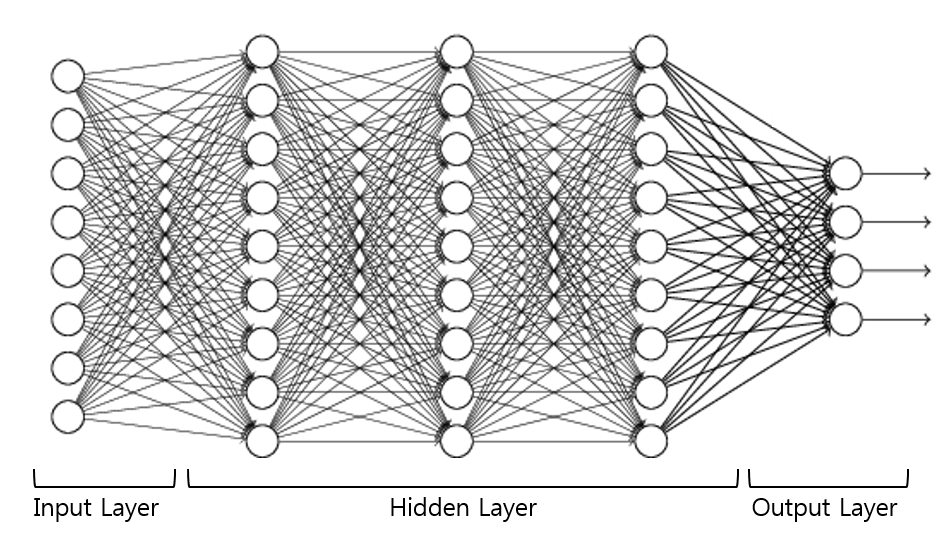
\includegraphics[width=9cm]{figures/three_hidden_layers.png}
		\caption{A neural network with three hidden layers.}
	\end{figure}
	There are three \textbf{hidden layers} to the network--i.e., three sequence of 
	convolution/pooling/ReLU. The input for each sequence is the output for the one before it. As data 
	gets passed from one sequence to another, features increase in both number and specificity.

	The last component of the CNN is the fully-connected layer, which transforms the information from 
	the last convolution/pooling/ReLU sequence into predictors for, in this case, a regression model 
	(more specifically, softmax regression). The output of this model is a vector of the form (0, 1) or (1, 
	0), depending on whether the image is predicted to be an ``X'' or an ``O'' respectively. The 
	parameters of this model are automatically determined during training, just as the filters are. 
	
	The process that allows the CNN to set these parameters is known as \textbf{backpropagation}. The 
	training process of a CNN involves using it to predict whether certain images that are already known 
	to be  ``X'' or ``O'' are so.  \textbf{Training loss} can then be found by comparing the predictions of 
	the model with the truth. In broad terms, backpropagation is the means by which ``responsibility'' 
	for loss is attributed to different parts of the network. By an optimization function, these parts, 
	which can be filters and weights, are changed. This process continues until the end of training, by 
	which time loss should stabilize.
	
	\hspace*{-6mm}\textbf{Managing the presets}
	
	While much of the CNN is tuned automatically, its fundamental structure, or architecture, must be 
	preset before training. These presets are known as \textbf{hyperparameters}, and can significantly 
	affect the success of the training of the network. An example of a hyperparameter is the 
	\textit{learning rate}, which controls how significantly the aforementioned optimization function 
	alters the filter weights and other parameters at every step of the training process:
	\vskip 5mm
	\begin{figure}[h]
		\centering
		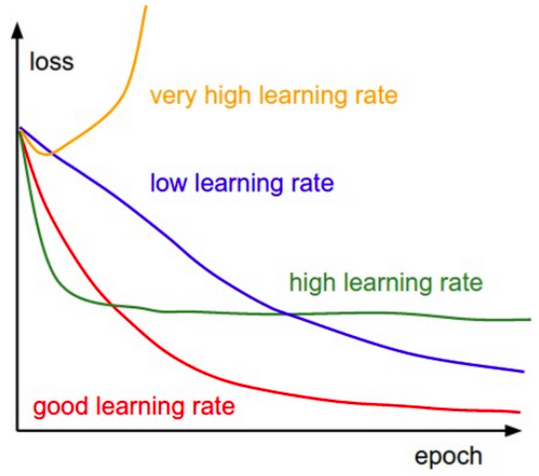
\includegraphics[width=5.5cm]{figures/learning_rates.png}
		\caption{A sketch of the reduction in training loss over time of different training 
			sessions, differentiated by learning rate~\cite{learning-rates}\relax.}
	\end{figure}
	
	Other hyperparameters include the number of hidden layers to be included in the model, the size of 
	the filters used, how many times each input image is to be used for training, etc. The process of 
	finding an architecture that is suitable for the problem at hand involves trial-and-error through 
	observation of the above training loss plot: if the training loss stabilizes at a sufficiently-low 
	level by the end of training, we are satisfied.
	
	The final evaluation of the model occurs after its training; the CNN is used to make predictions on 
	what is known as the ``test set''. This set also comprises of images that are known to be either ``X'' 
	or ``O'', meaning the CNN's predictions can be compared to the truth to ascertain its 
	\textit{testing accuracy}, i.e. predictive ability. In most contexts, a respectable testing accuracy can 
	be as high as 99+\%.
 
\section{A reference point: \textit{PKLot}}
    Most academic approaches to this occupancy problem have not used CNNs, favoring other machine 
    learning algorithms~\cite{quickspot-paper}\relax; a part of our preliminary research involved 
    reference to de Almeida et al.'s (2015) article: ``PKLot--A robust dataset for parking lot 
    classification''. This section will discuss our uses of this work's findings and data. \\
    \textbf{Release of the \textit{PKLot} dataset}
    
    With this work, the \textit{PKLot} dataset was released in the public domain\footnote{This dataset 
    can be found at: 
    \hyperlink{https://web.inf.ufpr.br/vri/databases/parking-lot-database/}{https://web.inf.ufpr.br/vri/databases/parking-lot-database/}.}.
    It comprises of 695,899 images of parking spots taken from two parking lots over the course of 
    about 30 days, in which there was great variation of weather and illumination 
    \cite{pklot-paper}\relax. We used this dataset to train and test CNNs that can classify spots as 
    either ``empty'' or ``occupied''; a further discussion of this process and its results will take place 
    soon. We have also used this dataset to understand workflow concerning organization, storage, and 
    labeling of images for the purposes of classification. The following are three example images from 
    this dataset:
	\vskip 5mm
    \begin{figure}[h]
        \centering
        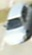
\includegraphics[width=1cm]{figures/example_1.jpg}
        \caption{An occupied spot from the first parking lot, in sunshine.}
        \vspace{5mm}
        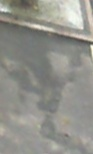
\includegraphics[width=1cm]{figures/example_2.jpg}
        \caption{An empty spot from one angle of the second parking lot, in overcast conditions.}
        \vspace{5mm}
        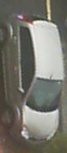
\includegraphics[width=1cm]{figures/example_3.jpg}
        \caption{An occupied spot from the second angle of the second parking lot, in rain.}
    \end{figure}

    \hspace*{-6mm}\textbf{Evaluation of the use of Support Vector Machines}
    
    The article also details the use of Support Vector Machines to classify spots, and evaluates their 
    performance under different training and testing schedules. We used this information to decide 
    which schedule to use for creating our CNNs. We decided to ascertain the testing accuracy 
    of 
    our CNNs using images only from the one parking lot which was used to train them. There were 
    other 
    alternatives that could be considered, such as training with the images of all parking lots before 
    testing on the images of one; however, it was found that the selected schedule is the 
    most performant. Moreover, in our future use-case of serving user requests for the occupancy of a 
    specific lot, we thought it less important to train the CNNs on a general dataset to later only use it 
    more 
    specifically.
        
    Therefore, a CNN for each of the three subsets (recall there are two parking lots, with images for 
    one taken at two angles) was created. The CNNs were implemented using 
    \href{https://www.tensorflow.org}{TensorFlow}, an efficient deep-learning library written for the 
    Python programming language. We picked TensorFlow for its efficiency, wide use and support, and 
    integration with  
    \href{https://www.tensorflow.org/programmers_guide/summaries_and_tensorboard}{TensorBoard}, a 
    tool which allows us to visualize the state of our model in great detail.
    
    Training  of the CNNs was done online on \href{https://www.floydhub.com}{FloydHub}. FloydHub is 
    a Platform-as-a-Service that quite inexpensively offers a pre-configured environment on powerful 
    hardware for ML purposes. Users run ``jobs'' through a command-line client, with data and 
    algorithms stored on Floydhub. Training metrics and logs are also stored on the cloud: 
    \vskip 5mm
    \begin{figure}[h]
    	\centering
    	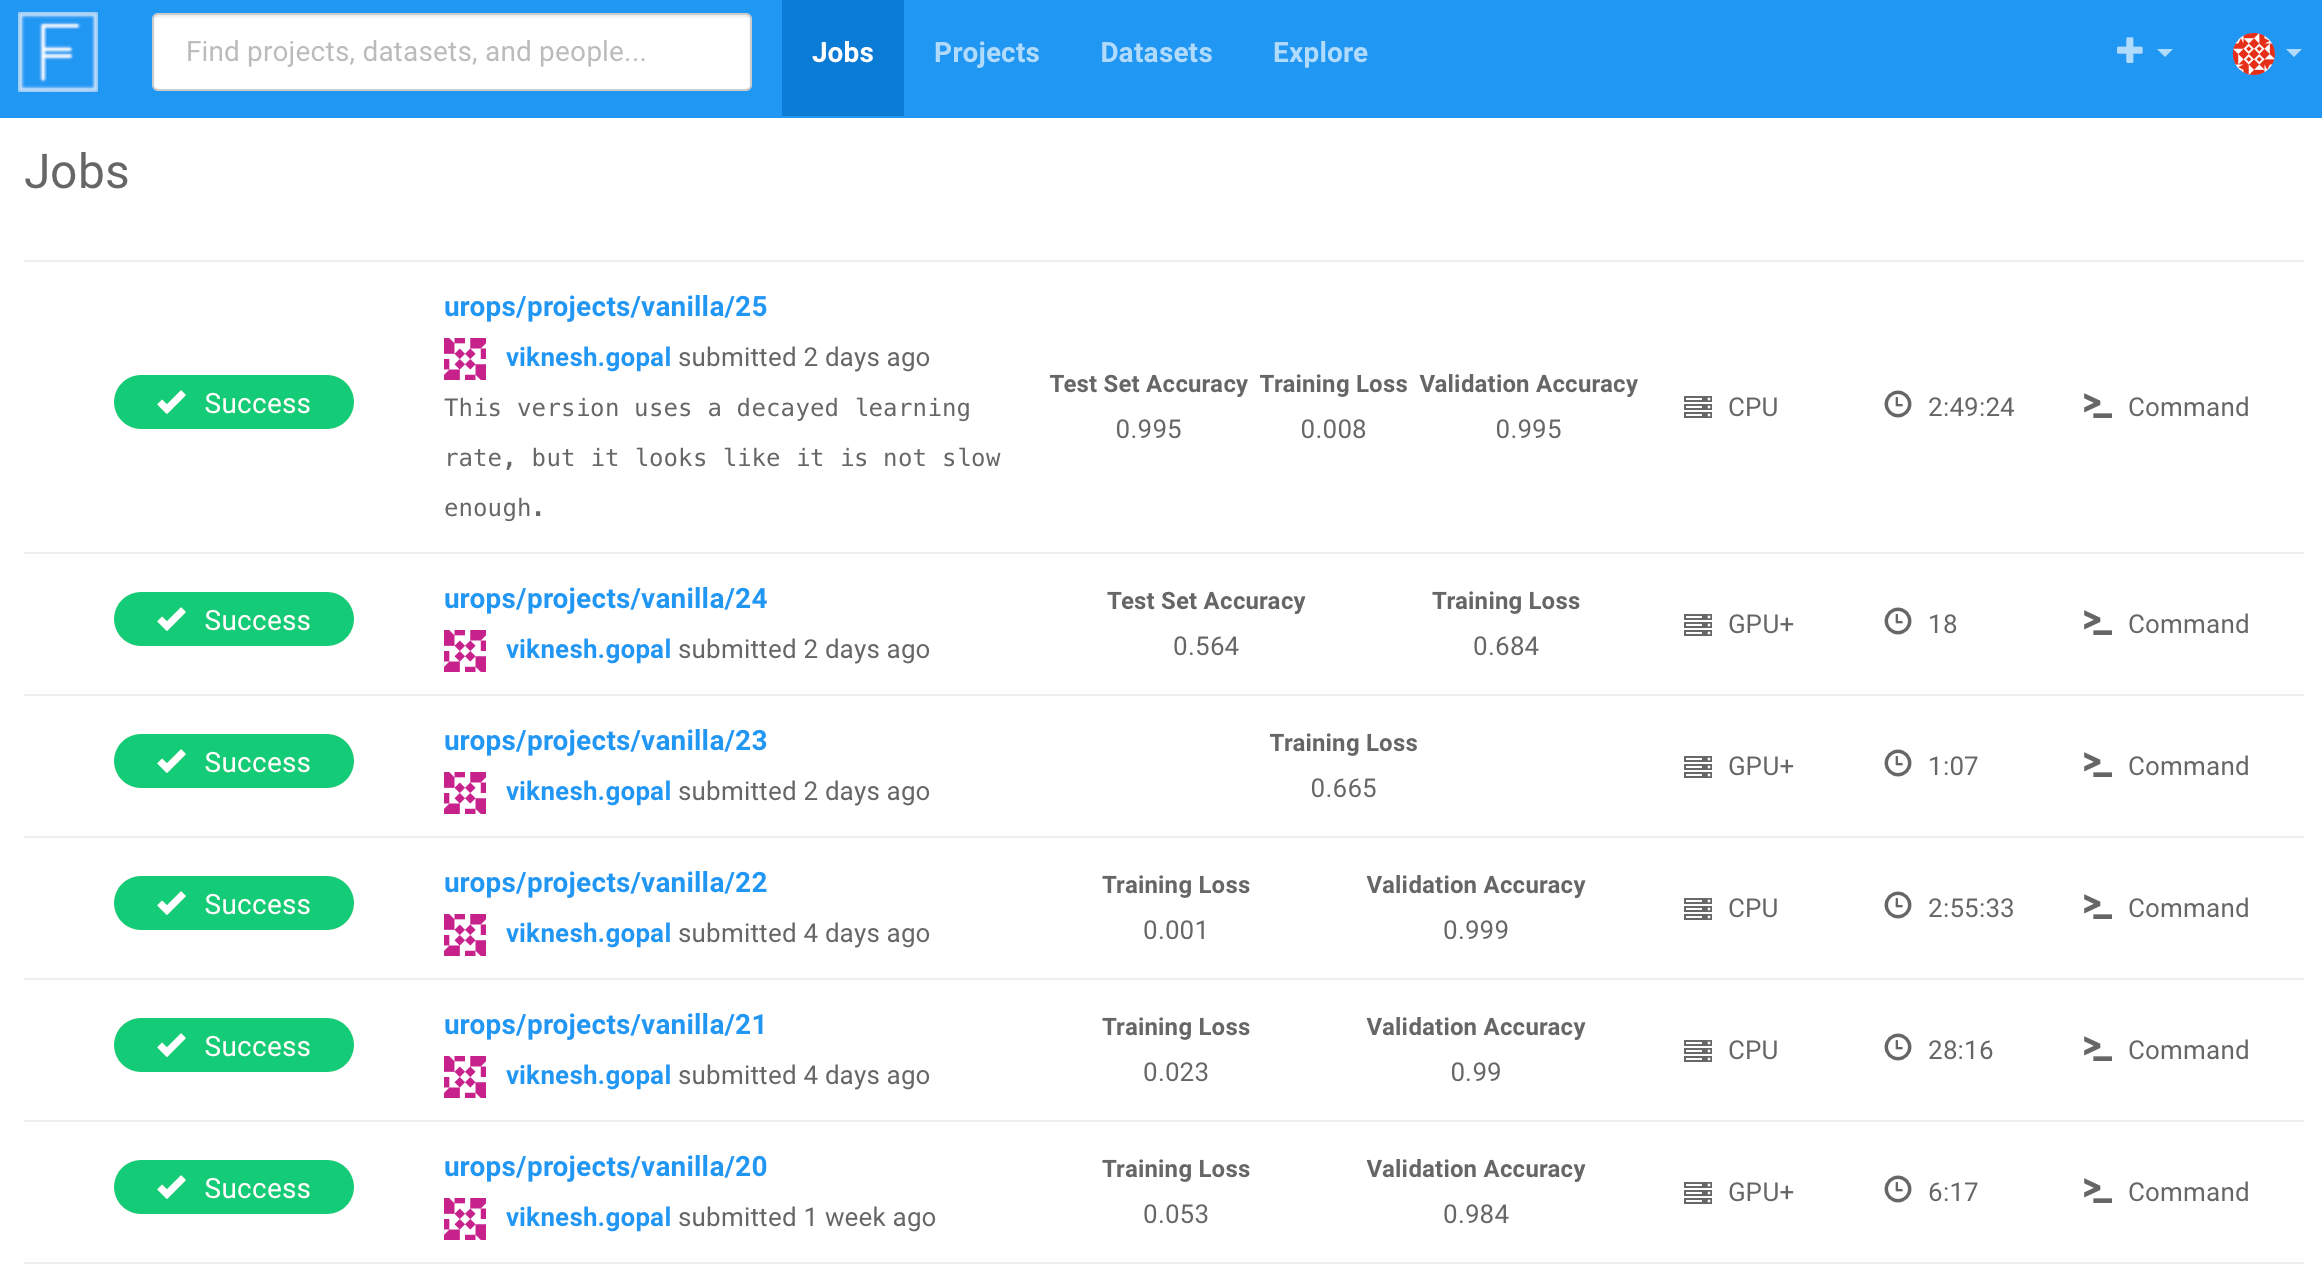
\includegraphics[width=14cm]{figures/floydhub.png}
    	\caption{Log of jobs run on FloydHub.}
    \end{figure}
    
    \newpage
    
    There are a number of reasons why we chose FloydHub: 
	\begin{enumerate}
		\item TensorFlow is set up and updated automatically for users on FloydHub along 
		with all dependency modules. 
		\item Great computing power is available on the cloud inexpensively; it saves us many hours 
		in training.
		\item Training multiple configurations of the same CNN concurrently is possible--on a personal 
		computer, it is not. Again, time is saved.
		\item Working on the cloud allows all involved in the project to collaborate seamlessly, and is the 
		norm in industry.
		\item Moving development to the cloud better prepares us to serve the model to users in future.
		\item FloydHub offers version control for files we upload to their servers.
	\end{enumerate}
	
	Each of our CNNs achieved a testing accuracy of 99.8+\%, which translates to the misclassification 
	of about 260 spots in requesting for the prediction of the state of about 175,000. It is therefore 
	without question that CNNs are apt tools for this task. The following was their architecture:
	\begin{itemize}
		\item[] An input layer which reads in 32-by-32 color images of parking spots.
		\item[] Convolutional layer 1: applies 32 5-by-5 filters, and then applies the ReLU activation 
		function.
		\item[] Pooling layer 1: performs max pooling with a 2-by-2 filter.
		\item[] Convolutional layer 2: applies 64 3-by-3 filters, and then applies the ReLU activation 
		function.
		\item[] Pooling layer 2: performs max pooling with a 2-by-2 filter.
		\item[] Fully-connected layer 1: comprises of 1,024 neurons/predictors.
		\item[] Output layer: 2 neurons, representing the output vector.
		\vspace*{-4mm}
		\begin{enumerate}
			\setlength\itemsep{-3mm}
			\item[] (1, 0) $\rightarrow$ occupied spot
			\item[] (0, 1) $\rightarrow$ empty spot
		\end{enumerate}
	\end{itemize}

	It will be fruitful to understand how this success can be replicated in the local context, where we 
	have control over collection of data.

\section{Future plans}

	This project is to be extended into the summer. There are two key objectives that will be worked 
	towards:
	\begin{enumerate}
		\item Construction of an Arduino-based camera to take pictures of an NUS parking lot over the 
		course of about thirty days, in the manner of \textit{PKLot}. Then, to clean, label, securely store, 
		and use this data to create CNNs.
			\begin{adjustwidth}{6mm}{}
				Doing so will help us understand the practical challenges involved in the collection of  
				data appropriate for our use: such challenges could pertain to security, infrastructure, 
				environment,  etc.
			\end{adjustwidth}
		\item Creation of a mobile application capable of serving the users of at least one NUS parking lot 
		in the following manner:
			\begin{center}
				User requests for spot-wise occupancy status through the application. \\
				$\downarrow$ \\
				Picture of lot taken by a standard CCTV or dedicated camera, \\
				and transmitted to associated cloud-based CNN. \\
				$\downarrow$ \\
				Spots in picture classified as empty or occupied by model. \\
				$\downarrow$ \\
				Picture deleted, and user sent spatially-accurate abstraction of spot-wise
				occupancy status (possibly in the manner pictured below).
			\end{center}
		\end{enumerate}
	
		\begin{figure}[h]
			\centering
			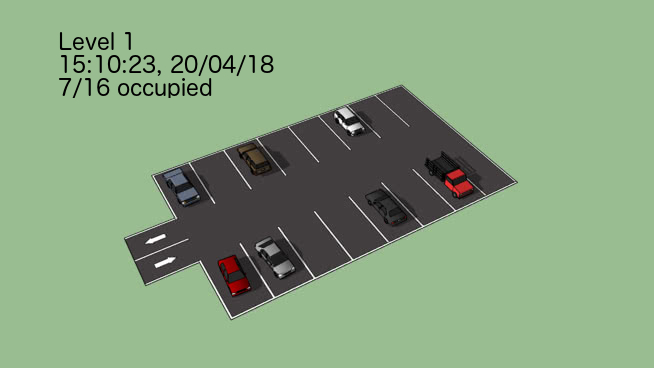
\includegraphics[width=8cm]{figures/mock-up.jpg}
			\caption{This visual could be delivered to users through the mobile application.}
		\end{figure}
		\newpage
		The first objective is to be addressed soon: an Arduino-based camera is being prepared and will 
		likely be gathering data through the month of May. This device will comprise of the following parts:
		\begin{enumerate}
			\item Arduino Uno (an inexpensive microcontroller).
			\item A five-megapixel camera module.
			\item 64 GB microSD card.
			\item Rechargeable 5200 mAh battery (with a protective sleeve).
		\end{enumerate}

		We have taken inspiration from \textit{PKLot} in the creation of the data collection schedule: a 
		picture of the selected parking lot will be taken every five minutes during working hours over the 
		course of thirty days. This will total to about 2,880 pictures. Given that there are about 50 spots 
		in the selected lot, we will have about 140,000 examples to train and test our CNN on, after images
		of 	individual spots have been extracted from the pictures in the manner of figures 14, 15, and 16. 
		We intend to gather such a large number of examples because many issues that prevent neural 
		networks from training well are related to a lack of training examples.
		
		Our selected parking lot is that belonging to block S17 at the Faculty of Science. Pictures will be 
		taken from a sufficiently-high vantage such that images cannot be used to identify people and car 
		plates. Moreover, as soon as pictures are taken, they will be encrypted using 256-bit AES 
		(Advanced Encryption Standard). This encryption helps protect the data against malicious 
		individuals who attempt to steal the device. Moreover, the device will be regularly visited: given 
		estimates of energy consumption, batteries will have to be replaced about every five days. After 
		the data collection has finished, pictures will be deleted from the microSD card and transferred to 
		FloydHub, where files can be accessed only by uploaders. FloydHub also uses 256-bit AES to 
		communicate with local machines to run jobs. They have taken measures to restrict the number of 
		users (to just two) who have administrative access to their servers. Finally, user passwords and 
		authentication tokens are not managed by them, but by Auth0. We believe this is more than 
		sufficient for our application and data.
		
		\hspace*{-6mm}The following is visual context to our data collection:
		\vskip 5mm
		\begin{figure}[h]
		    \centering
		    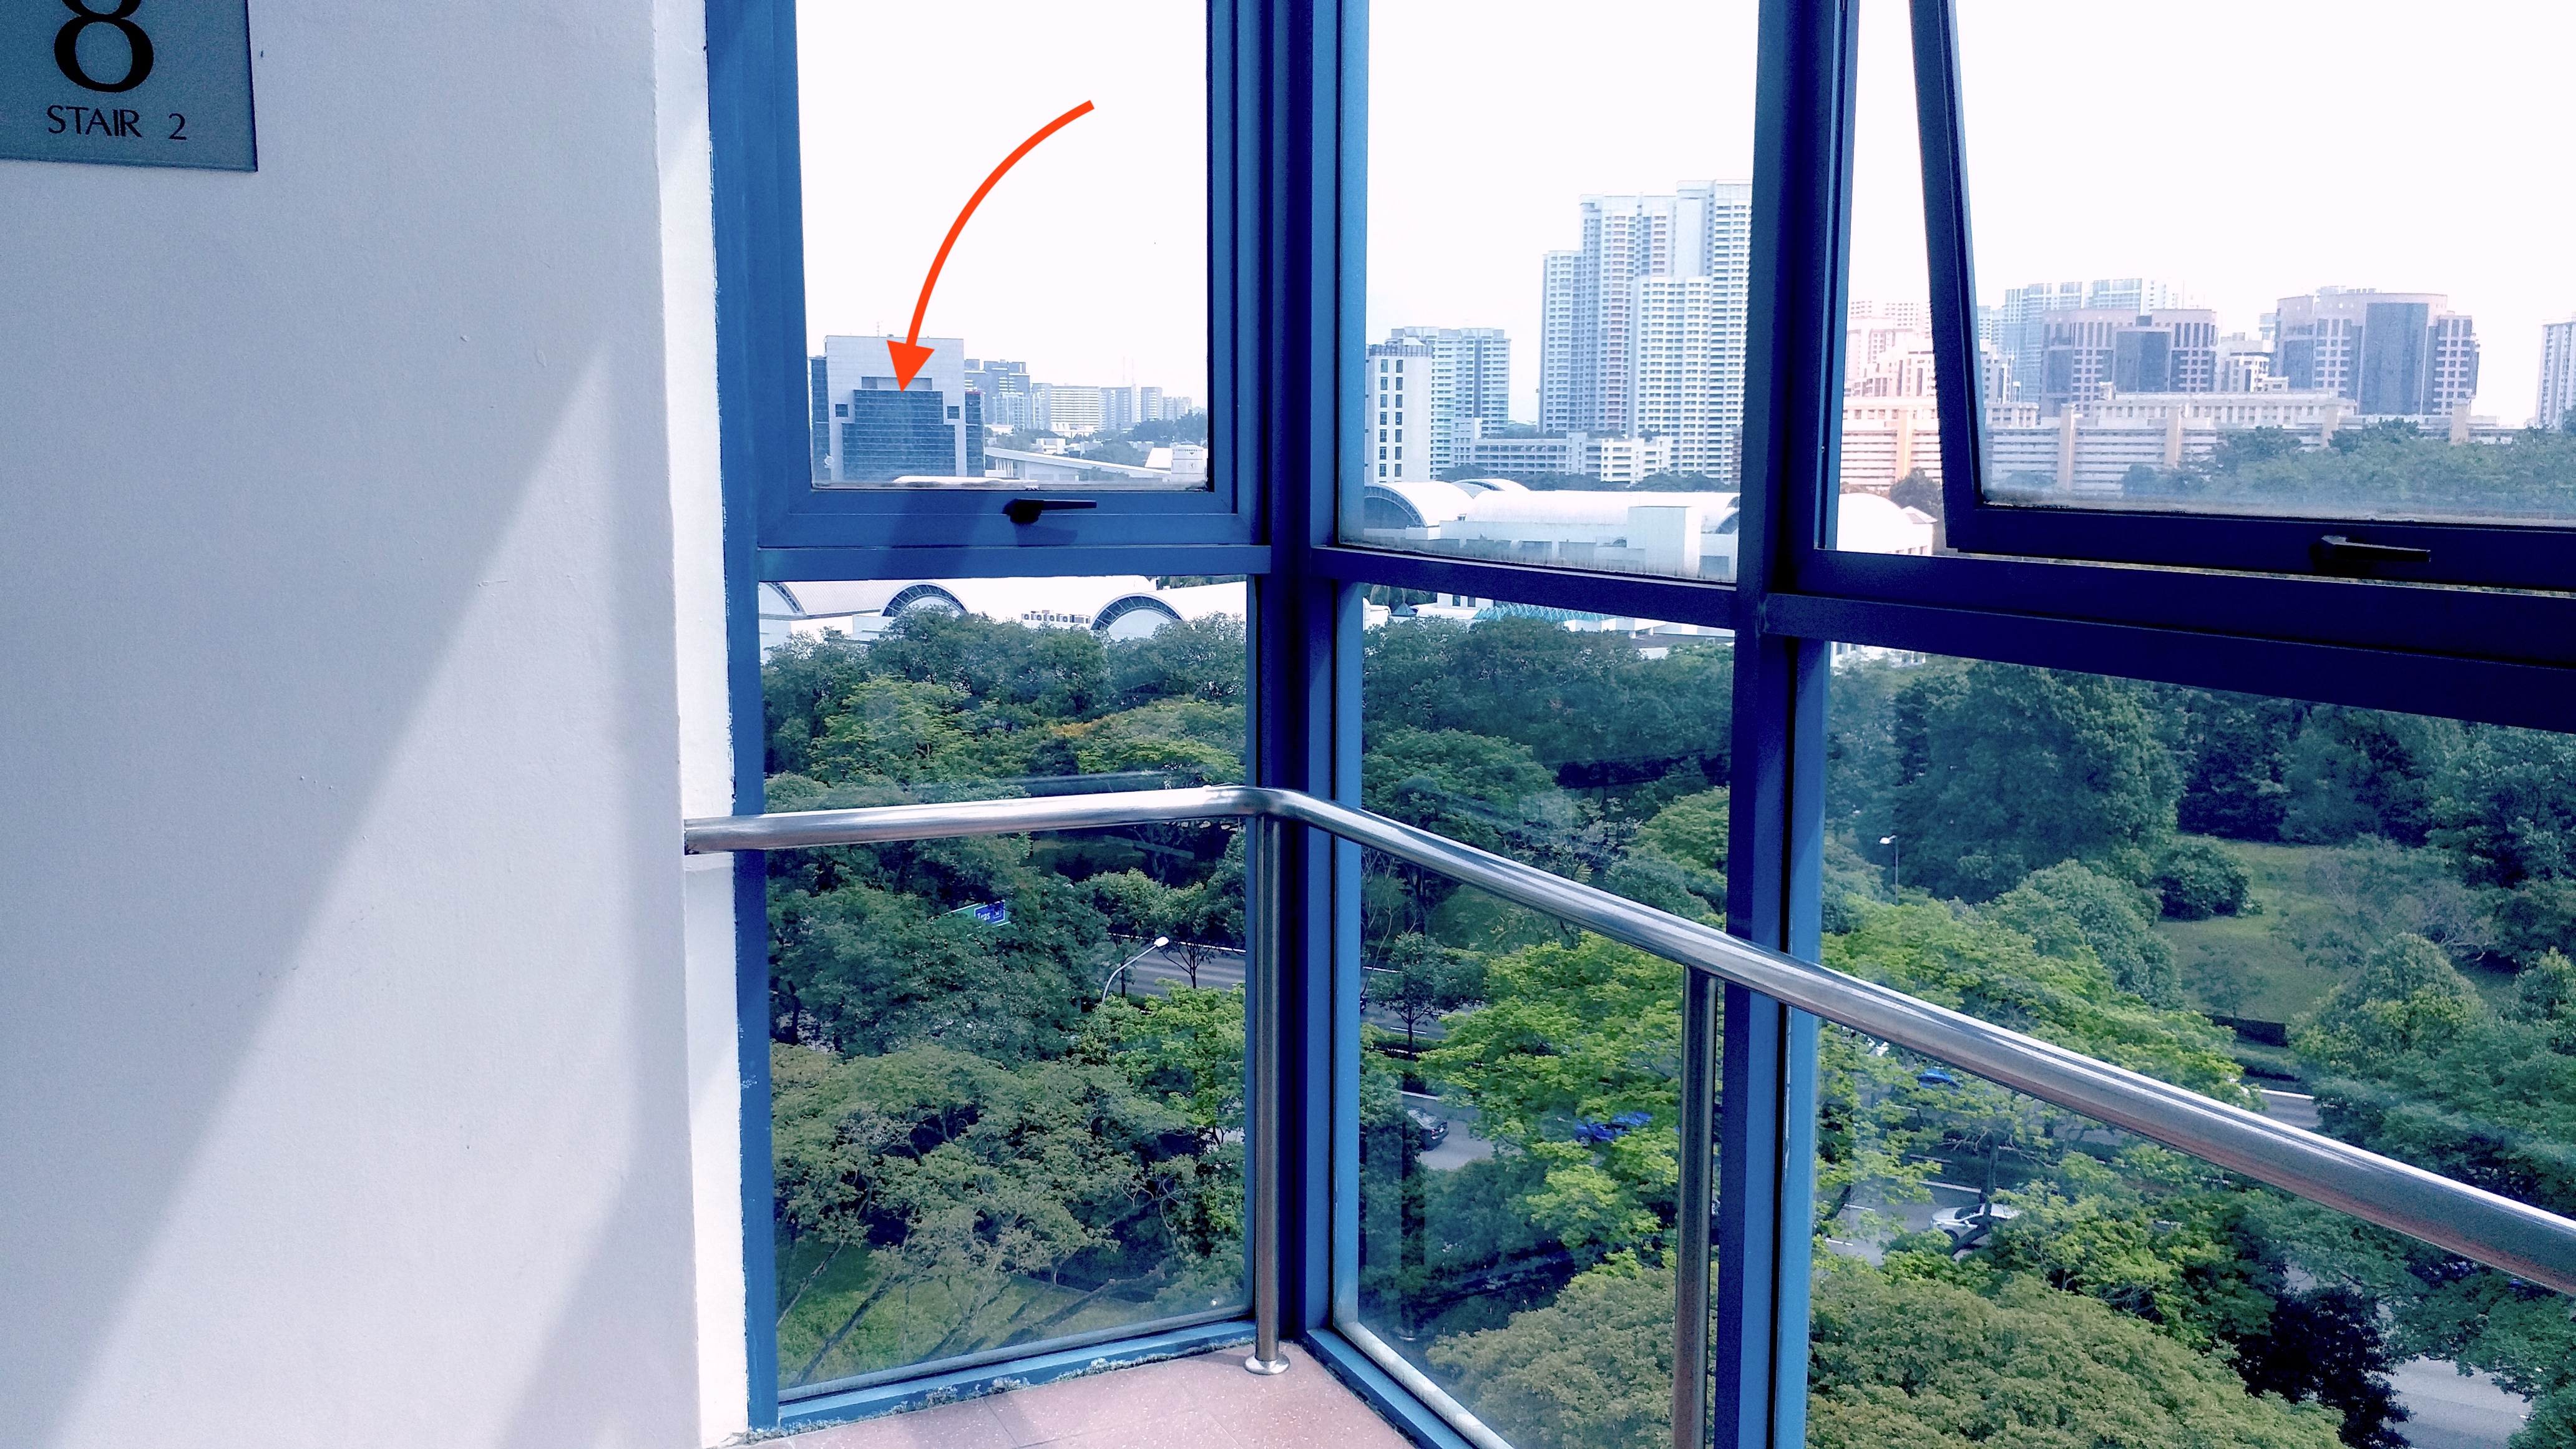
\includegraphics[width=0.4\textwidth]{figures/context_used.jpg}
		    \caption{The Arduino-camera will be mounted on this window,}
		\end{figure}
	
		\begin{figure}[h]
			\centering
			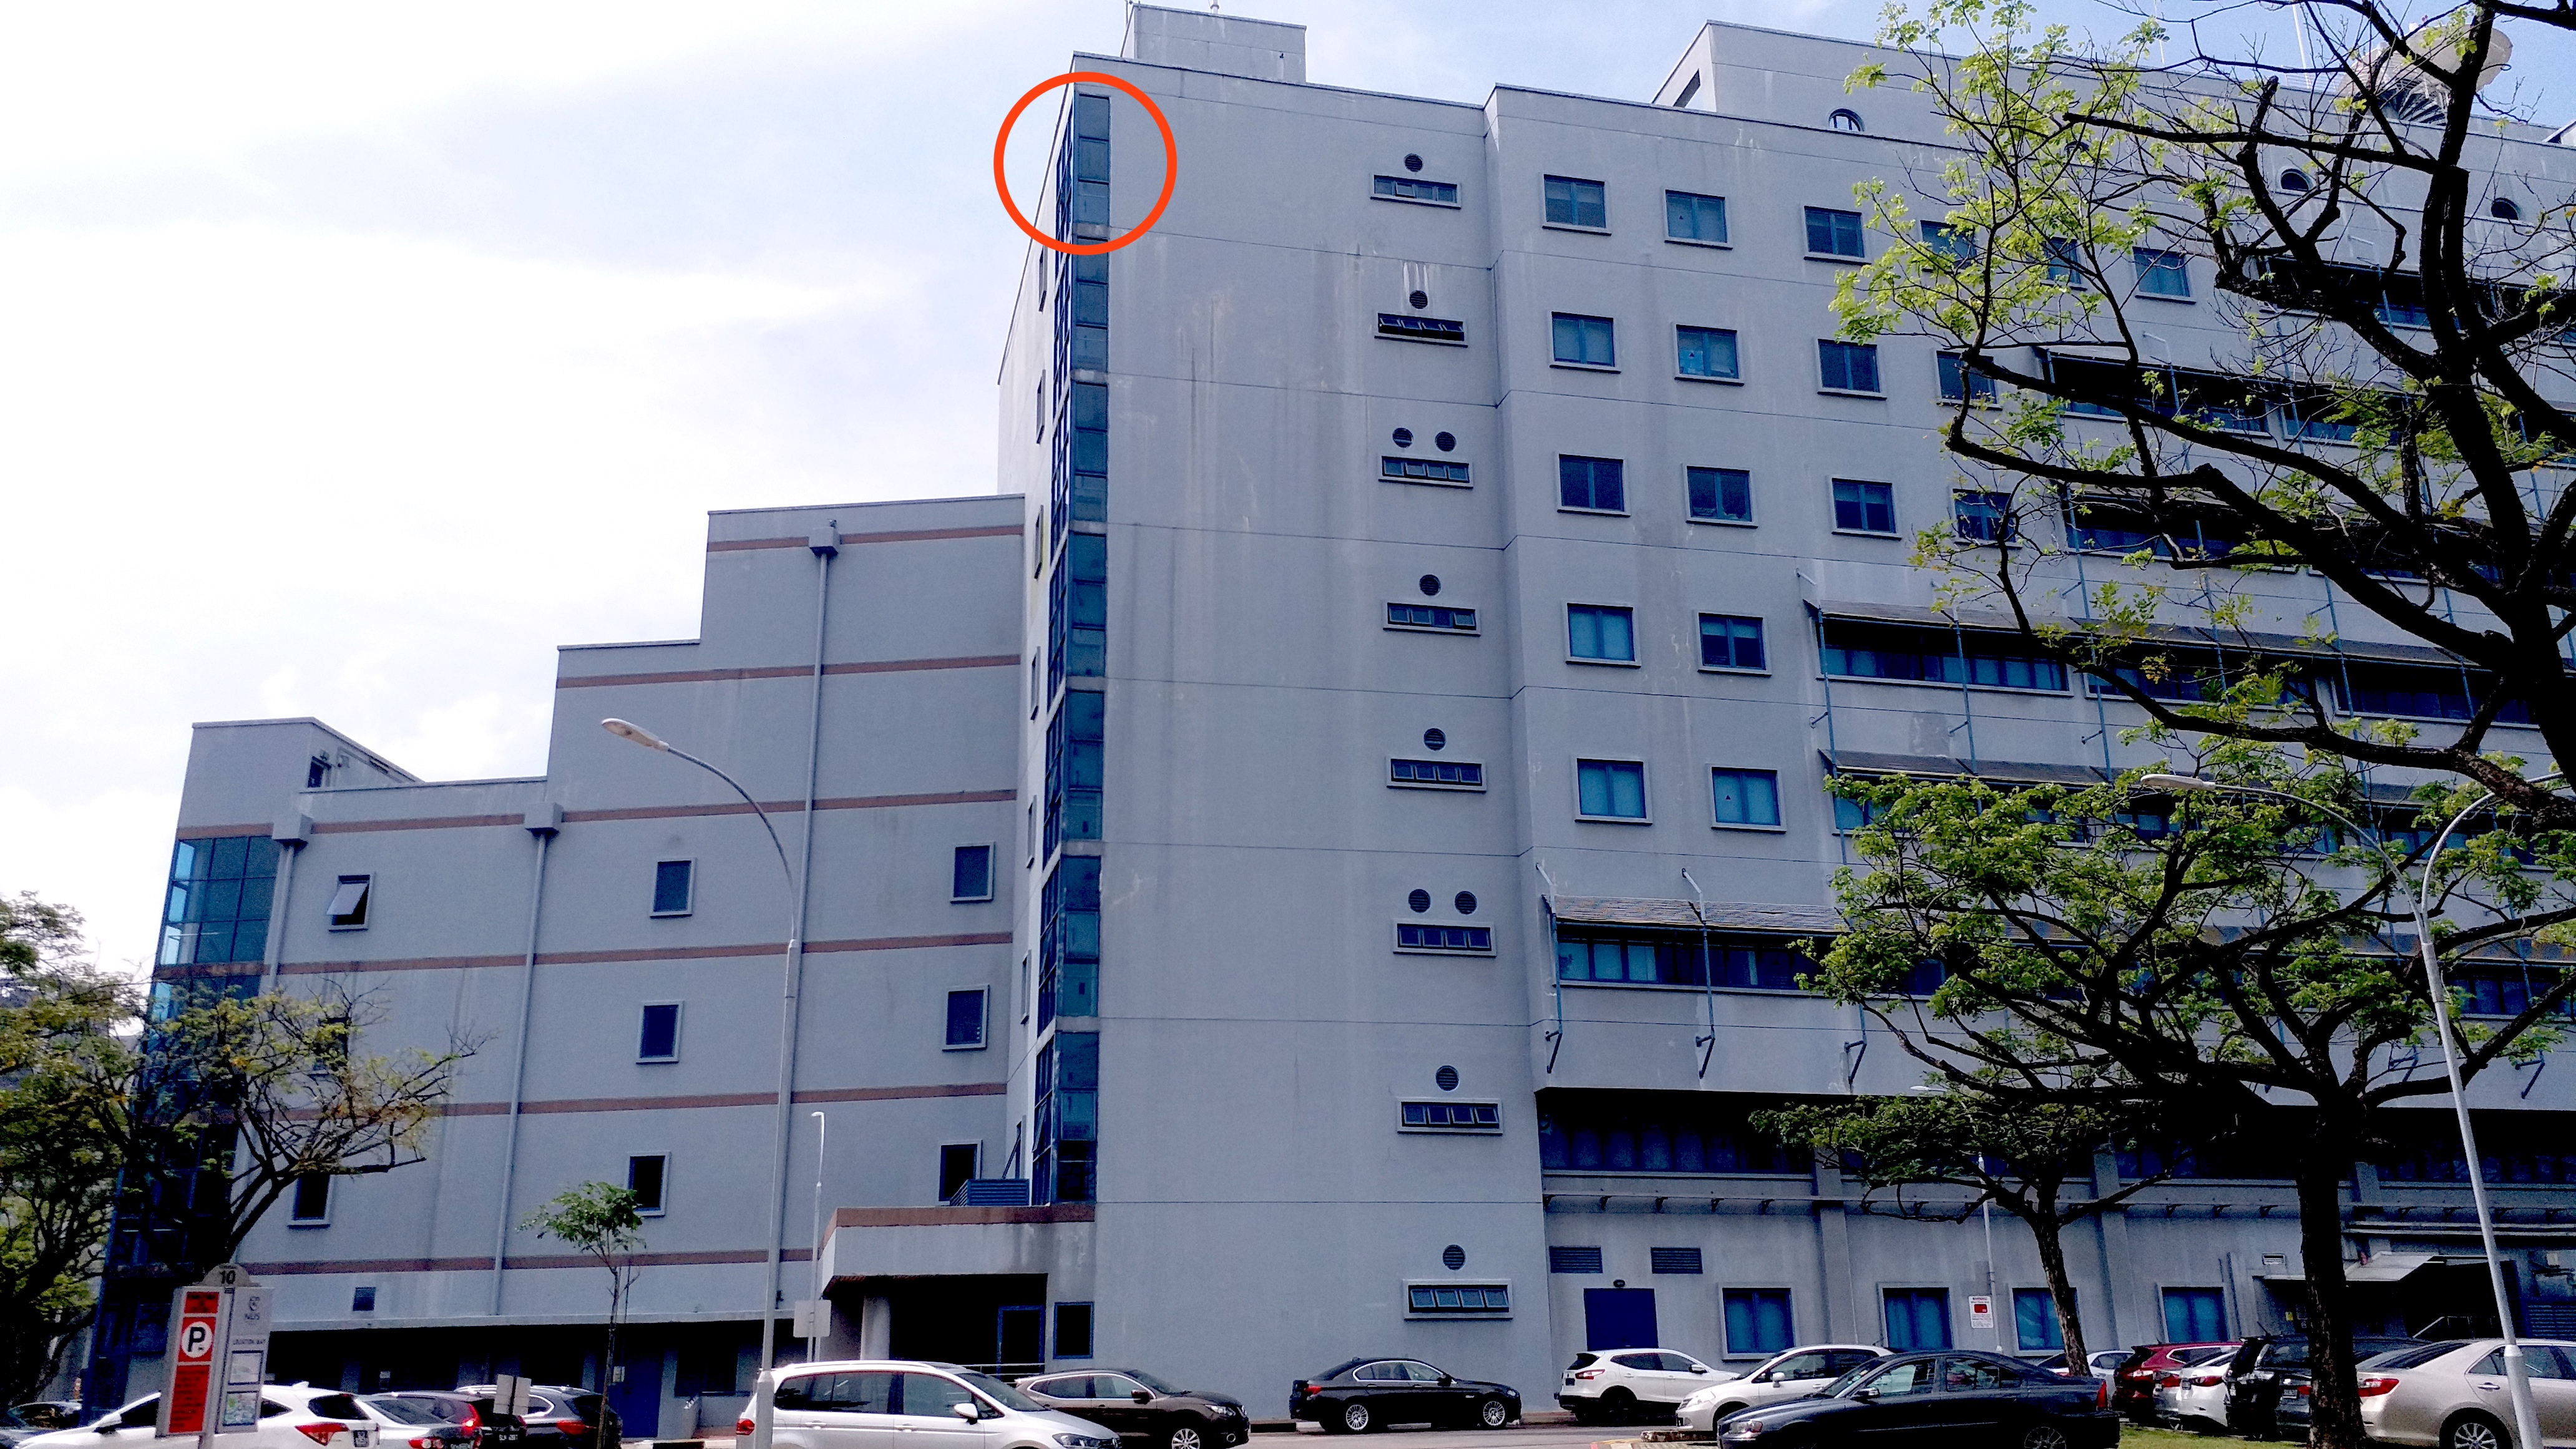
\includegraphics[width=0.4\textwidth]{figures/context2_used.jpg}
			\caption{located at the encircled position,}
			\vskip 5mm
		    \includegraphics[width=0.4\textwidth]{figures/view_full.jpg}
		    \caption{facing the following parking lot.}
		\end{figure}
		\newpage
		The approach to the second objective, creation of the mobile application, is dependent on the 
		experiences from the first. Namely, the second objective will require upgrade of the camera to one 
		that is Internet-connected; powering and reliably connecting such a device can be challenging. 
		Moreover, the CNN will need to be placed on the cloud, with a suitable interface to handle 
		communication between the camera(s) taking the picture upon user request, the model serving 
		the prediction, and the user's mobile application. Amazon's Amazon Web Services offers us tools 
		to host CNNs on the cloud~\cite{aws}\relax. They offer serverless services that can scale 
		dynamically in capacity in response to demand, and are only billed per user request. Our 
		application intends to harness such services in its back-end.
		
\section{Conclusion and extensions}
	The use of CNNs to ascertain the occupancy of parking lots has shown good promise, and is soon 
	to be applied to the local context. Nonetheless, increasing the resolution of information available to 
	those seeking a parking spot is not the only implication of this project, especially given that NUS' 
	parking lots are organized appropriately for demand. Rather, we truly view this project as a 
	capability-building exercise; a segue into greater problems that can be addressed by machine 
	learning--either by us or those who take reference to our experiences in the future. For instance, 
	even in the context of this application, there are several extensions that we could consider:
	\begin{enumerate}
		\item How well can we classify the lots using grayscale images, which is typically what we obtain 
		from CCTV cameras?
		\item How well can we classify lots at night?
		\item How can we overcome occlusion due to trees or neighbouring large cars?
		\item How well can the model perform this task indoors? How extensive a network of cameras 
		would be needed in such a case?
	\end{enumerate}

%\newpage

\begin{thebibliography}{unsrt}
    \bibitem{pklot-paper}
		Almeida, P. R., Oliveira, L. S., Britto, A. S., Silva, E. J., \& Koerich, A. L. (2015). PKLot--A robust 
		dataset for parking lot classification. \textit{Expert Systems with Applications}, 42(11), 
		4937-4949. doi:10.1016/j.eswa.2015.02.009
	\bibitem{pict-num}
		Chapter 1. Digital image representation. (n.d.). Retrieved April 20, 2018, from 
		http://pippin.gimp.org/image\_processing/chap\_dir.html
	\bibitem{learning-rates}
		CS231n Convolutional Neural Networks for Visual Recognition. (n.d.). Retrieved April 19, 2018, 
		from http://cs231n.github.io/neural-networks-3/
	\bibitem{conv-pool-viz}
		Dumoulin, V., \& Visin, F. (2018). A guide to convolution arithmetic for deep learning. A Guide to
		Convolution Arithmetic for Deep Learning. doi:1603.07285v2 (arXiv)
	\bibitem{aws}
		Ivanovic, B., \& Ivanovic, Z. (2017, December 29). How to Deploy Deep Learning Models with AWS 
		Lambda and Tensorflow. Retrieved April 19, 2018, from 
		http://awscentral.blogspot.com/2018/01/how-to-deploy-deep-learning-models-with.html
	\bibitem{brain-analogy}
		Liljeqvist, I. (2016, March 20). The Essence of Artificial Neural Networks. Retrieved April 19, 2018, 
		from https://medium.com/@ivanliljeqvist/the-essence-of-artificial-neural-networks-5de300c995d6
    \bibitem{quickspot-paper}
		M\`armol, E., \& Sevillano, X. (2016). QuickSpot: A video analytics solution for on-street vacant 
		parking spot detection. Multimedia Tools and Applications, 75(24), 17711-17743. 
		doi:10.1007/s11042-016-3773-8
	\bibitem{architecture}
		Navoshta, A. (2017, January 15). Traffic signs classification with a convolutional network. 
		Retrieved April 20, 2018, from https://navoshta.com/traffic-signs-classification/
	\bibitem{filter-viz}
		Pavlovsky, V. (2017). Introduction To Convolutional Neural Networks. Retrieved April 20, 2018, 
		from http://www.vaetas.cz/posts/intro-convolutional-neural-networks/
    \bibitem{parking-sensors}
		Robarts, S. (2015, September 29). Bosch sensor connects parking spaces to the Web. Retrieved 
		April 19, 2018, from https://newatlas.com/bosch-active-parking-lot-management/39629/
	\bibitem{cnn-working}
		Rohrer, B. (2016, August 18). How do Convolutional Neural Networks work? Retrieved April 20, 
		2018, from https://brohrer.github.io/how\_convolutional\_neural\_networks\_work.html
	\bibitem{use-of-relu}
		S. (2018, February 26). Why do we use ReLU in neural networks and how do we use it? 
		[https://stats.stackexchange.com/q/226927].
    \bibitem{pollution-paper}
        Shoup, D. C. (2006). Cruising for parking. \textit{Transport Policy, 13}, 479-486. doi:10.1016/j.tranpol.2006.05.005
	\bibitem{convol-filter}
		Spatial Enhancements. (n.d.). Retrieved April 20, 2018, from 
		http://gsp.humboldt.edu/olm\_2015/Courses/GSP\_216\_Online/lesson4-2/spatial.html

\end{thebibliography}

\end{document}